\documentclass[12pt]{exam}
\usepackage[utf8]{inputenc}

\usepackage[margin=1in]{geometry}
\usepackage{amsmath,amssymb}
\usepackage{multicol}
\usepackage{mathrsfs}
\usepackage{amsmath}
\usepackage{graphicx}
\usepackage{wrapfig}
\usepackage{tikz}
\usepackage{forest}
\tikzset{
  tree node/.style = {align=center, inner sep=0pt, font = \scriptsize},
  S/.style = {draw, circle, minimum size = 8mm, top color=white, bottom color=black!20},
  tree node label/.style={font=\scriptsize},
}
\forestset{
  declare toks={left branch prefix}{},
  declare toks={right branch prefix}{},
  declare toks={left branch suffix}{},
  declare toks={right branch suffix}{},
  tree node left label/.style={
    label=180:#1,
  },
  tree node right label/.style={
    label=0:#1,
  },
  maths branch labels/.style={
    branch label/.style={
      if n=1{
        edge label={node [left, midway] {$\forestoption{left branch prefix}##1\forestoption{left branch suffix}$}},
      }{
        edge label={node [right, midway] {$\forestoption{right branch prefix}##1\forestoption{right branch suffix}$}},
      }
    },
  },
  text branch labels/.style={
    branch label/.style={
      if n=1{
        edge label={node [left, midway] {\foresteoption{left branch prefix}##1\forestoption{left branch suffix}}},
      }{
        edge label={node [right, midway] {\forestoption{right branch prefix}##1\forestoption{right branch suffix}}},
      }
    },
  },
  text branch labels,
  set branch labels/.style n args=4{%
    left branch prefix={#1},
    left branch suffix={#2},
    right branch prefix={#3},
    right branch suffix={#4},
  },
  set maths branch labels/.style n args=4{
    maths branch labels,
    set branch labels={#1}{#2}{#3}{#4},
  },
  set text branch labels/.style n args=4{
    text branch labels,
    set branch labels={#1}{#2}{#3}{#4},
  },
  branch and bound/.style={
    /tikz/every label/.append style=tree node label,
    maths branch labels,
    for tree={
      tree node,
      S,
      math content,
      s sep'+=30mm,
      l sep'+=15mm,
      thick,
      edge+={thick},
    },
    before typesetting nodes={
      for tree={
        split option={content}{:}{tree node left label,content,tree node right label,branch label},
      },
    },
    where n children=0{
      tikz+={
        \draw [thick]  ([yshift=-10pt, xshift=-2.5pt].south west) -- ([yshift=-10pt, xshift=2.5pt].south east);
      }
    }{},
  },
}
\usepackage{tikz-qtree}
\usetikzlibrary{calc, shapes}

\newcommand{\class}{SA 405}
\newcommand{\term}{Fall 2018}
\newcommand{\examnum}{Final Exam}
\newcommand{\examdate}{Dec 14, 2018}
\newcommand{\timelimit}{180 Minutes}

\pagestyle{head}
\firstpageheader{}{}{}
\runningheader{\class}{\examnum\ - Page \thepage\ of \numpages}{\examdate}
\runningheadrule

%% Answer box macros
%% \answerbox{alignment}{width}{height}
\newcommand{\answerbox}[3]{%
  \fbox{%
    \begin{minipage}[#1]{#2}
      \hfill\vspace{#3}
    \end{minipage}
  }
}

%% \answerboxfull{alignment}{height}
\newcommand{\answerboxfull}[2]{%
  \answerbox{#1}{6.38in}{#2} 
}

%% \answerboxone{alignment}{height} -- for first-level bullet
\newcommand{\answerboxone}[2]{%
  \answerbox{#1}{6.0in}{#2} 
}

%% special boxes
\newcommand{\wordbox}{\answerbox{c}{1.2in}{.7cm}}
\newcommand{\catbox}{\answerbox{c}{.5in}{.7cm}}
\newcommand{\letterbox}{\answerbox{c}{.7cm}{.7cm}}



\begin{document}

\noindent
\begin{tabular*}{\textwidth}{l @{\extracolsep{\fill}} r @{\extracolsep{6pt}} r}
\textbf{\class} &&\textbf{\examnum}\\
\textbf{\term} &&\textbf{\examdate}\\
 && \\
 && \\
\textbf{Midshipmen are persons of integrity.}& \textbf{Name:} & \makebox[2.2in]{\hrulefill}\\\\
\textbf{Time Limit: \timelimit} %& Teaching Assistant & \makebox[2in]{\hrulefill}
\end{tabular*}

\noindent
\rule[2ex]{\textwidth}{2pt}

%This exam contains \numpages\ pages (including this cover page) and \numquestions\ questions.\\
%Total of points is \numpoints.

\begin{itemize}
\item Do {\bf not} write your name on each page, only write your name above.

\item No books or notes % or calculators
% that do symbolic manipulation (such as TI-89 or TI-92) 
 are allowed. %{\bf One} 8.5 by 11 inch formula/note sheet is allowed.

%\item You may use your calculator on this test.

\item Show all work clearly. (Little or no credit will be given for a numerical
answer without the correct accompanying work.
Partial credit is given where appropriate.) 

%\item If you need more space than is provided, use the back of the previous page. 

\item Read each question carefully.
If you are not sure what a question is
asking, ask for clarification.

\item If you start over on a problem, CLEARLY indicate what your final
  answer is, along with its accompanying work.

%\item All formulations must have descriptions of any indices, parameters, and decision variables used. All constraints must be described. 
\end{itemize}


\begin{center}
Grade Table (for teacher use only)\\
\addpoints
\gradetable[v][questions]
\end{center}

\noindent
\rule[2ex]{\textwidth}{2pt}

\newpage %%%%%%%


\begin{questions}

%%% Network Flow, Fixed charge, Set covering, Logical constraints %%%
\question \label{ques:shortestpath} The Superintendent asks you and your OR classmate to give him directions from the Yard to Naval Base San Diego, the principal homeport of the Pacific Fleet. 
Of course, he wants to find the path that minimizes his total travel time, but he has a few more requirements: he only wants to pass through cities that have Navy Lodges, and he never wants to drive more than eight hours at a stretch between cities. 

\begin{center} 

\includegraphics[width = 0.4\textwidth]{usna_to_nbsd}
\end{center}

\smallskip

Your classmate defines the following sets and parameters:

\bigskip
\renewcommand{\arraystretch}{1}
\begin{tabular}{lcl}
$\mathcal{C}$ & $:=$ & the set of cities in the United States that have Navy Lodges; \\
\\
$\mathcal{A}$ & $:=$ & the set of routes $(i,j)$ from city $i$ to city $j$, for $i, j$ in $\mathcal{C}$, such that the \\
&& drive time from $i$ to $j$ is no more than 8 hours; \\
\\
$t_{i,j}$ & $:=$ & the drive time from city $i$ to city $j$, for all $(i,j)$ in $\mathcal{A}$;\\
$a$ & $:=$ & the element of $\mathcal{C}$ representing Annapolis;\\
$s$ & $:=$ & the element of $\mathcal{C}$ representing San Diego.\\
\end{tabular}

\bigskip
\begin{parts}

\part [10] Picking up where your partner left off, write a mathematical program in \textbf{abstract} form whose solution solves the Superintendent's routing problem.  Clearly define any additional notation that you use.

\newpage
\fullwidth{Question \ref{ques:shortestpath}, continued.}
\part [4]  Additional research reveals that due to traffic, traveling through many of the cities $i \in \mathcal{C}$ incurs delays, and your classmate defines the parameters,

\smallskip
\begin{tabular}{lcl}
$d_i$ & $:=$ & the extra time required if driving through city $i$, for all $i \in C$.
\end{tabular}

\smallskip
Adjust your model to incorporate city delays.  Again, clearly define any additional notation that you use.

\vfill\vfill

\part  After you brief the Superintendent on the optimal route, he makes a few requests due to the locations of various friends and relatives.   Use the variables you have already defined to add constraints to the model that will enforce the Superintendent's latest requests.
\begin{subparts}
\subpart[2] He definitely wants to visit city 10, but not city 11. \vfill
\subpart[2] He wishes to visit at least one of cities 3, 4 and 5.  \vfill
\subpart[2] If he visits cities 3 and 4, he definitely does not want to visit city 5. \vfill
\end{subparts}

\end{parts}

\newpage
\question \label{ques:vrp} Your regional manager at Dunder Mifflin, Michael Scott, has asked you to solve a \textbf{Vehicle Routing Problem (VRP)} to determine an optimal set of 3 paper-delivery routes for delivering paper to their 9 customers. He assumes that each route begins and ends at their warehouse in Scranton, PA. Mr. Scott's goal is to minimize the total distance traveled among all vehicles. 

Each delivery route must be used, must visit at least two customers, and can transport no more than 425 cases of paper. Assuming that all distances are symmetrical, the table below gives the distances between the warehouse (WH) and each of the 9 customers.

\begin{table}[h]
\caption{Distances between the warehouse and all customers.}
\begin{center}
\begin{tabular}{|c|c|c|c|c|c|c|c|c|c|c|}
\hline
& WH &1&2&3&4&5&6&7&8&9\\ \hline
WH & - &10&12&13&40&25&16&37&23&19 \\ \hline
1& -  & - & 12 & 23 & 14 & 17 & 11 & 7 & 34 & 21 \\ \hline
2& -  & -  & - & 13 & 24 & 28 & 16 & 9 & 8 & 19 \\ \hline
3& -  & -  & -  & - & 24 & 26 & 14 & 13 & 12  & 5 \\ \hline
4& -  & -  & -  & -  & - & 5 & 37 & 17 & 8 & 9 \\ \hline
5&-  & -  & -  & -  & -  & - & 16 & 4 & 18 &  21 \\ \hline
6& -  & -  & -  &-  & -  & -  & - & 27 & 11 &  13 \\ \hline
7& -  & -  & -  & -  & -  & -  & -  & - & 18 & 9 \\ \hline
8& -  & -  & -  & -  &-  & -  &-  & -  & - & 19 \\ \hline
9& -  & -  & -  &-  & -  & -  & -  & -  & -   &- \\ \hline
\end{tabular}

\end{center}
\end{table}

\begin{table}[h]
\caption{Demand (in number of cases of paper) for each customer}
\begin{center}
\begin{tabular}{|c|c|}
\hline
Customer&Demand\\ \hline
1 & 20  \\ \hline
2 & 80  \\ \hline
3 & 90 \\ \hline
4 &  120\\ \hline
5 & 110 \\ \hline
6&  150\\ \hline
7& 100  \\ \hline
8& 75 \\ \hline
9& 85 \\ \hline
\end{tabular}

\end{center}
\end{table}
\newpage
\fullwidth{Question \ref{ques:vrp}, continued.}

\begin{parts}
\part[10] Provide an \emph{abbreviated} \textbf{concrete} integer programming model for solving Mr. Scott's problem above. Clearly define your variables. Provide your objective function and all constraints required to solve Mr. Scott's problem. You can omit any subtour-elimination and route-splitting constraints in this formulation. \medskip \\

\newpage
\fullwidth{Question \ref{ques:vrp}, continued.}
\part[5] You solve the problem, and your solution thankfully contains no subtours. In this solution, vehicle 1 visits the sequence of customers $(1,6)$, vehicle 2 visits the sequence of customers $(2,4,5,7,8)$ and vehicle 3 visits the sequence of customers $(3,9)$. Is this solution feasible? If so, provide a brief explanation why. If not, provide the appropriate set of constraints to eliminate this infeasible solution.\medskip \\
\vfill
\part[5] Michael Scott tells you that each vehicle can now only travel up to 80 miles along an entire delivery route. Compared to the original problem (without this travel distance maximum), do you expect the optimal objective function value for this new problem to increase, decrease, or remain the same? Give a brief explanation with your answer. \medskip \\
\vfill

\end{parts}

\newpage

\question \label{ques:fl}  There is currently an outbreak of the Ebola virus in the Democratic Republic of Congo (DRC). Given a limited budget, the World Health Organization (WHO) is looking to build temporary testing facilities that will be assigned to one or more cities to identify who has been infected in those cities. WHO's task is determine which of the testing facilities should be built to maximize the total number of people in the DRC who have access to Ebola testing.

\smallskip
Sets \& Parameters:

\begin{tabular}{lcl}
$C$ & $:=$ & the set of cities in the DRC; \\
$F$ & $:=$ & the set of possible testing facilities in the DRC; \\
$N_c$ & $:=$ & ($\subseteq F$) the set of facilities in $F$ that could serve city $c \in C$;
\\
\\
$p_{c}$ & $:=$ & the population of city $c \in C$;\\
$t_f$ & $:=$ & the cost of building testing facility $f \in F$ in American dollars;\\
$b$ & $:=$ & the budget of the WHO in American dollars.\\
\end{tabular}

Variables:

\begin{tabular}{lcl}
$x_c \in \{0,1\}$ & $:=$ & $1$ if city $c \in C$ is served, $0$ otherwise.\\
$y_f \in \{0,1\}$ & $:=$ & $1$ if testing facility $f \in F$ is built, $0$ otherwise.\\
\end{tabular}

\medskip

\begin{parts}
\part[12] Use the sets, parameters, and variables defined above to formulate an \textbf{abstract} mathematical programming model to maximize the total number of people tested for Ebola in the DRC without exceeding the WHO's budget. Clearly define all variables, present an objective function, and present all appropriate constraints.\medskip
\\
\vfill

\newpage
\fullwidth{Page left blank intentionally.}

\newpage
\fullwidth{Question \ref{ques:fl}, continued.}
\part[8] To be more fiscally-minded, WHO decides to change their objective. Instead of maximizing the total number of people who have access to testing, WHO decides to minimize the total cost of building testing facilities as long as $D$ number of people have access to Ebola testing.  Rewrite your integer program to model this problem.  \emph{(No need to redefine variables that you have already defined in part (a).)} \medskip
\\
%\vfill
%\part[4] Finally, the WHO changed their strategy again. They are now seeking to minimize the total cost of building testing facilities so that \textbf{all} people in the DRC have access to Ebola virus testing. Please provide any additional constraint(s) to model this change.\medskip \\
%\vfill

\end{parts}



\newpage
\question Given the graph $G$ in Figure \ref{primsfigure} below, execute Prim's algorithm to calculate a minimum spanning tree. Show your steps in the table, as described below.

	\begin{figure}[h] 
	\label{primsfigure}
	\center
	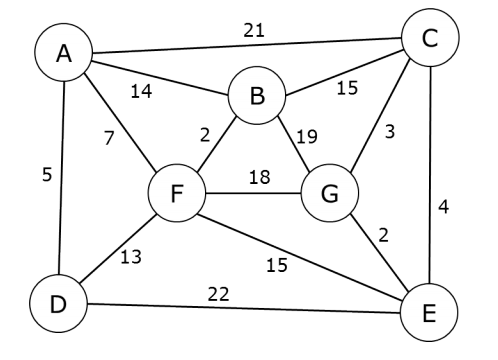
\includegraphics[width=0.45\textwidth]{prims_picture}
	\caption{Graph $G$}
	\end{figure}

\begin{parts}

\part [15]  For each iteration, provide all nodes currently in $S$ (at the beginning of the iteration), all edges in the cut-set $C_{S, \bar{S}}$, and the edge that should be added to the minimum spanning tree $T$.  Start at vertex A.  Break any ties alphabetically.

\vspace{-15pt}
\arraycolsep=10pt
\def\arraystretch{2.5}
\[
\begin{array}{|c|c|c|c|}
\hline
\text{Iteration} &\qquad  \text{Set } S \qquad    &  \qquad \qquad \text{Cut-set } C_{S,\bar{S}}	\qquad \qquad &	\text{Add edge to } T \\ \hline
1 & &  &  \\ \hline
2 & & & \\ \hline
3 & & & \\ \hline
4 & & & \\ \hline
5 & & & \\ \hline
6 & & & \\ \hline
\end{array}
\]
\smallskip

\part [5]   Indicate the minimum cost spanning tree produced by the algorithm by highlighting its edges in graph $G$ above. Provide its cost below.
\end{parts}

\newpage

%%% Bellman-Ford %%%
\question Given the graph $H$ in Figure \ref{bellmanfordfig} below, execute the Bellman-Ford algorithm to determine a shortest path from node $1$ to node $6$. 

\begin{figure}[h]
	\label{bellmanfordfig}
	\center
	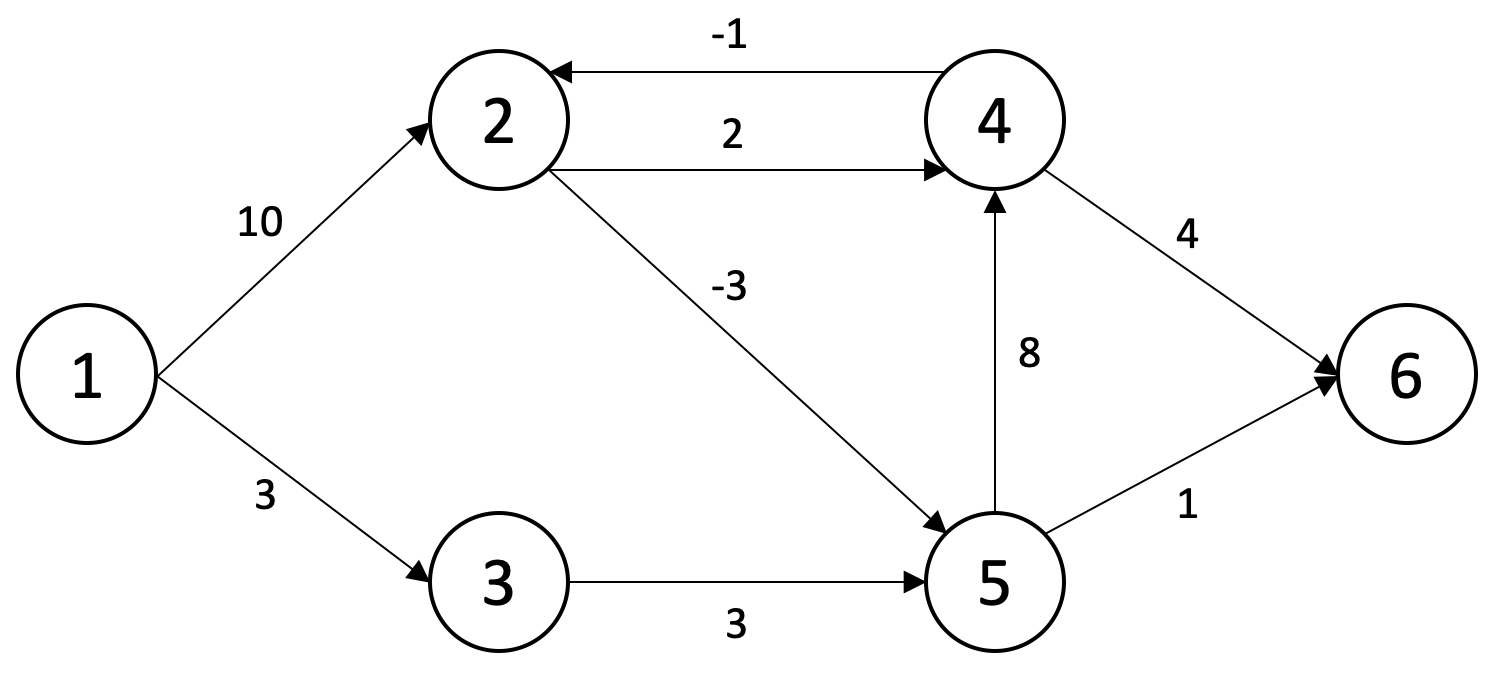
\includegraphics[width=8cm]{BellmanFordFigure}
	\caption{Graph $H$}
	\end{figure}

\medskip

Use the following ordering of edges to execute the algorithm:
\begin{align*}
& (1,2), \ (1,3), \ (2,4), \ (2,5), \ (3,5), \ (4,2), \ (4,6), \ (5,4), \ (5,6)
\end{align*} 

\begin{parts}
\part[10] Initialize each node with an appropriate distance label. Use the table below to track changes in distance labels, $d$, and predecessors, $pred$. Break any ties by choosing the minimum node label.

\arraycolsep=25pt
\def\arraystretch{1.5}
\[
\begin{array}{|c|c|c|c|c|c|c|}
\hline
\text{Vertex} & 1&2&3&4&5&6 \\
 \hline
d &  &  & & & &\\ 
 &  &  & & & &\\ \hline
pred & & & & & &\\ 
 &  &  & & & &\\ \hline
\end{array}
\]


\medskip \medskip
\part[5] Provide the final vector of distance labels $d$ and the final vector of predecessor labels $pred$.
\medskip \medskip
\begin{itemize}
\item[] $d = \{ \qquad  , \qquad , \qquad  , \qquad , \qquad , \qquad  \}$
\medskip \medskip
\item[] $pred = \{ \qquad , \qquad , \qquad  , \qquad , \qquad , \qquad  \}$
\end{itemize}

\medskip
\part [5] List the shortest path from node 1 to node 6 provided by the algorithm.

\end{parts}

%%% TU and Integrality, Option 1 %%%
\newpage
\question[10] We studied three different algorithms for optimizing on graphs, as listed below.  State the graph problem that each aims to solve, and whether or not the procedure is guaranteed to result in a globally optimal solution. 
\begin{itemize}
\item[] Nearest Neighbor:  \vfill

\item[] Prims: \vfill

\item[] Bellman-Ford:  \vfill
\end{itemize}


\question  
\begin{parts}
\part [6] Recall that a linear program (LP) in canonical form is as follows:
\begin{align*}
\textrm{max } & \mathbf{c}^T\mathbf{x} \\
\textrm{s.t. } & \mathbf{A}\mathbf{x}= \mathbf{b} \\
& \mathbf{x} \ge \mathbf{0}.
\end{align*}
List two requirements that together guarantee that all basic feasible solutions of a linear program in canonical form are integer-valued.
\vfill \vfill
\part [4] Describe a practical problem that can be modeled by an integer program whose continuous LP relaxation is guaranteed to provide an integer-valued optimal solution. % (It is ok to choose a problem that we did in the notes or in the homework.)
\vfill \vfill
\end{parts}



%%% TU and Integrality, Option 2 %%%
%\newpage
%\question 
%\begin{parts} 
%\part Is the following matrix totally unimodular?  Explain.
%\[ A =
%\begin{bmatrix}
%    1     & 0 &  1   \\
%      0     & 1 & -1 
%\end{bmatrix}
%\]
%\vfill
%
%\part  Describe a problem that can be modeled by a linear program with continuous variables that is guaranteed to have integer-valued solutions. 
%\vfill
%\end{parts}

%%% Convex-hull Formulation %%%
\newpage
\question Consider the integer program formulation provided and graphed below.

\begin{minipage}{.3\textwidth}
Formulation (I)
\begin{align*}
-5x + 3y &~\leq~ 0 \tag{A} \\
9x + 20y &~\leq~ 95 \tag{B} \\
20x + 3y &~\leq~ 90 \tag{C} \\
x, ~y & ~\ge~ 0, ~\text{integer}
\end{align*}
\end{minipage}\hspace{0.7cm}
\begin{minipage}{.5\textwidth}
\begin{center}
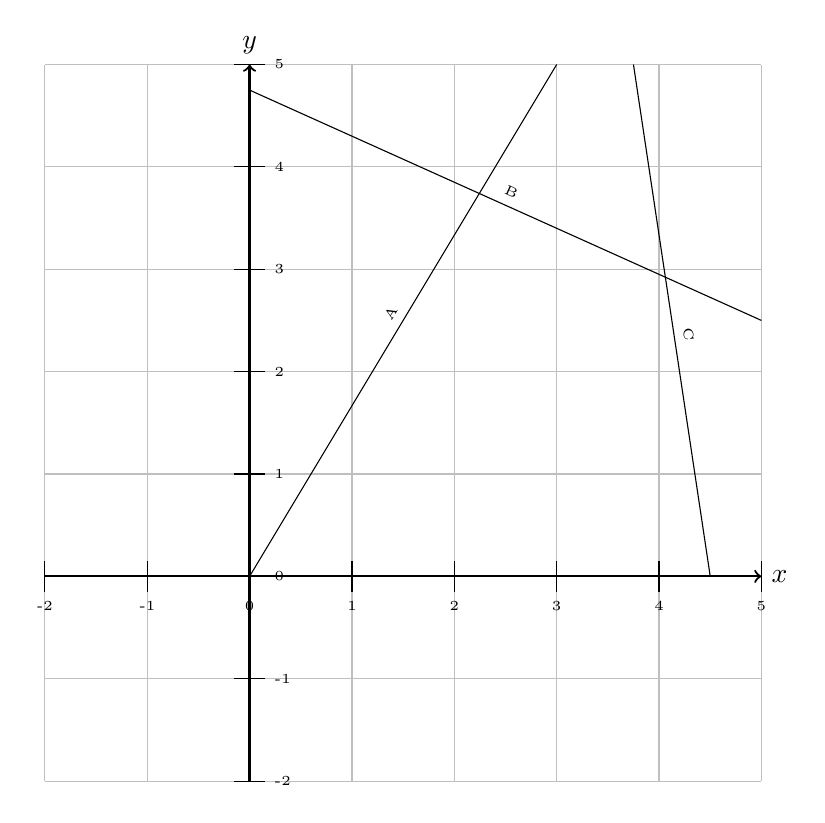
\begin{tikzpicture}[scale = 1.3]
  \draw[gray!50, thin, step=1] (-2,-2) grid (5,5);
  \draw[ thick,->] (-2,0) -- (5,0) node[right] {$x$};
  \draw[ thick,->] (0,-2) -- (0,5) node[above] {$y$};

 \foreach \x in {-2,...,5} \draw (\x,0.15) -- (\x,-0.15) node[below] {\tiny\x};
 \foreach \y in {-2,...,5} \draw (-0.15,\y) -- (0.15,\y) node[right] {\tiny\y};

  \draw (0,0) -- node[above,sloped]       {\tiny A}   (3,5);
  \draw (5,2.5) -- node[above,sloped]       {\tiny B} (0,4.75);
  \draw (4.5,0) -- node[above right,sloped] {\tiny C} (3.75,5);
\end{tikzpicture} 
\end{center}
\end{minipage}

\bigskip
\begin{parts}
\part [6] On the same graph, sketch the convex hull formulation, which we will call Formulation (II), of the integer feasible region described by Formulation (I).  List the inequalities that describe Formulation (II).

\vfill

\part [4] Which formulation is ``better'' for solving the associated integer program, Formulation (I) or Formulation (II)?  Explain.

\vfill
\end{parts}

\newpage


%%% Branch and Bound %%%
\newpage
\question  Consider the branch and bound tree provided below, as applied to a \emph{maximizing}, two-variable integer program with integer objective coefficients.  For each subproblem, the optimal objective value, $z$, and optimal solution, $(x, y)$, to its continuous (non-integer) relaxation is provided. At each node, let $z^*$ be the current upper bound on the \emph{integer subproblem} implied by the solution to its relaxation.

\vspace{-0.6cm}
\begin{center}
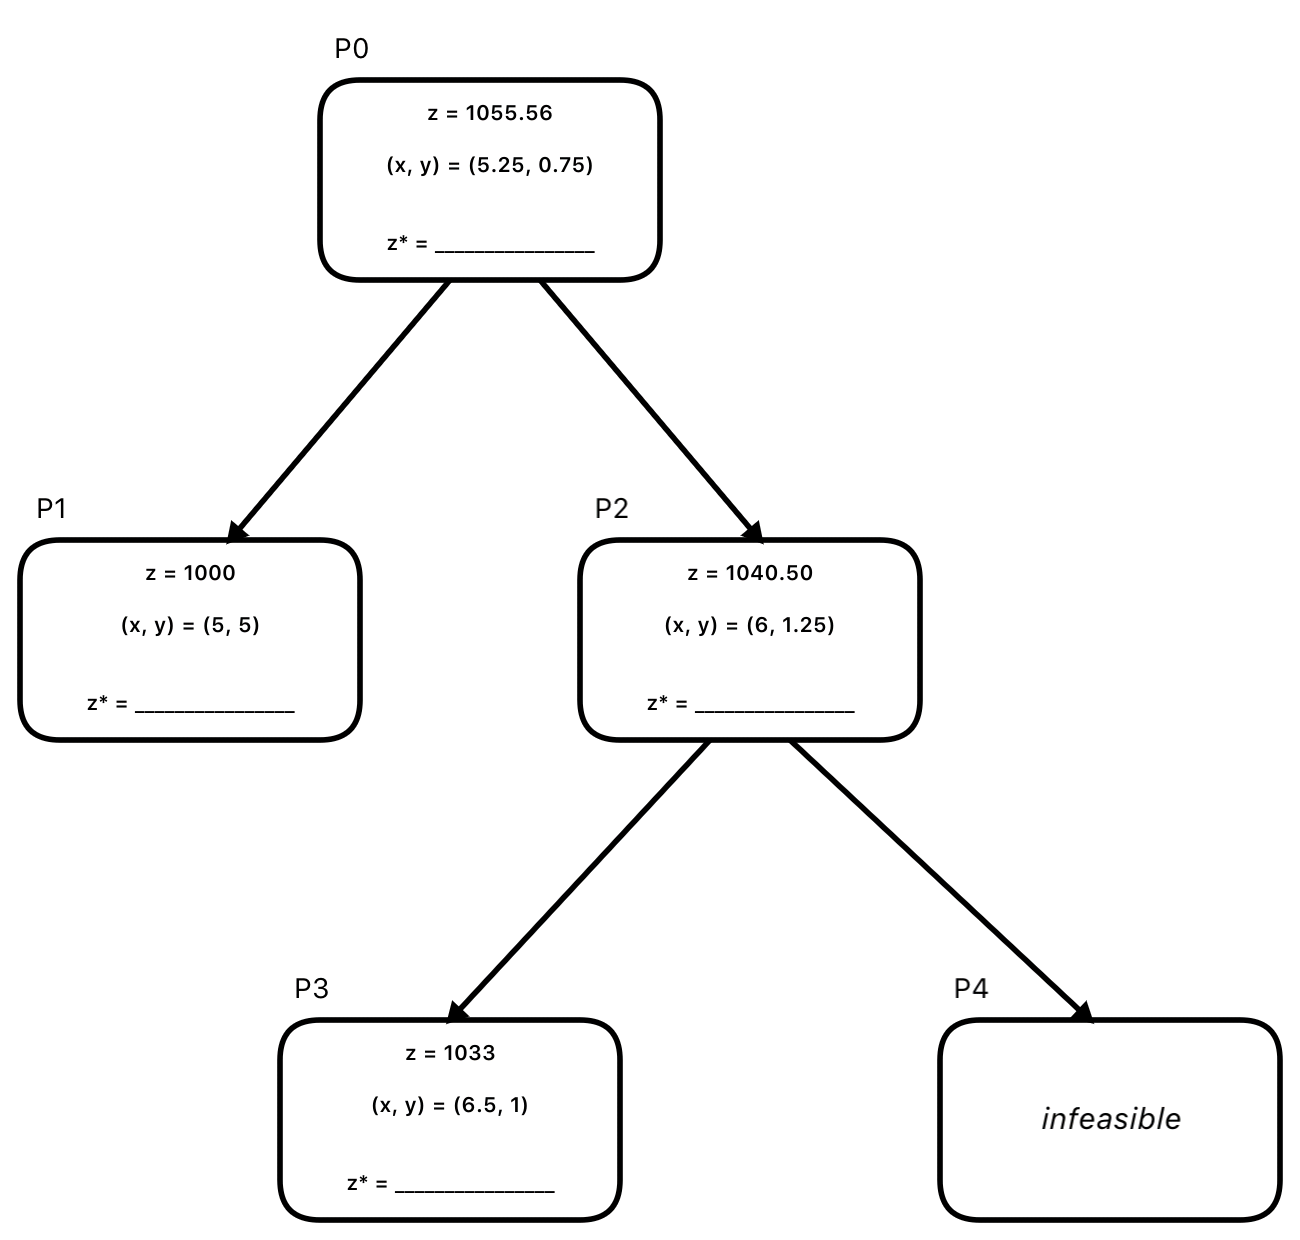
\includegraphics[width=0.7\textwidth]{bb_tree}
\end{center}

\begin{parts}
\part [4] Label each arrow with the constraint that is added to form the next subproblem.
\part [4] Fill in $z^*$ for each subproblem, the upper bound on the integer subproblem implied by $z$.
\part [6] Identify the incumbent solution, if one exists, as well as the best known upper bound and lower bound for the optimal objective value of the original problem, $P0$. \bigskip
\begin{center}
\begin{tabular}{c|c|c}
Incumbent solution & Global upper bound & Global lower bound \\
\hline
&& \\
&&
\end{tabular}
\end{center}

\bigskip
%\part List the incumbent solution, if applicable.
\part  [6] Is the branch and bound algorithm complete?\underline{\hspace{1.5cm}} ~ If so, provide the optimal solution.  If not, describe the next step.
\end{parts}

\end{questions}



\end{document}
